\chapter{Data and Experimental Setup} \label{chap:setup}

\section{Training, Calibration, and Testing}

\subsection{Data Construction} \label{sec:data_construction}
The dataset comprises responses from candidates taking the Linguaskill exams for second language (L2) \nomenclature[Z]{L2}{Second Language} learners of English. These exams are divided into five sections, each scored on a scale from 0 to 6. This study focuses on Part 1, where candidates answer eight questions about themselves \cite{linguaskills}. Candidates are provided 10 seconds to respond to the first four, and 20 seconds for the last four. The first two questions are not graded. Overall, the candidates' performance across all sections is mapped to CEFR levels ranging from A1 to C2 \cite{CEFR}.

For text-based model, the dataset contains the response transcripts extracted from the audio files. For feature-based model, the dataset contains the 356-dimensional features extracted from the audio files. For audio-based model, the dataset contains the audio represented in vector format. Each item in the dataset has an associated candidate number to identify the candidate, and the corresponding score from the human graders.

The dataset is divided into three sections: training, calibration, and testing. The training set is used to train the model, the calibration set is used to tune linear calibration after the score prediction from the neural network (Chapter \ref{chap:graders}), and the testing set is used to evaluate the model's performance. Table \ref{tab:data_size} shows the number of candidates in each section of the dataset.

\begin{table}[H]
    \centering
    \begin{tabular}{|c|c|c|}
        \hline
        \textbf{Training} & \textbf{Testing} & \textbf{Calibration} \\ \hline
        31471             & 1048             & 1033                 \\ \hline
    \end{tabular}
    \caption{Number of candidates in each section of the dataset}
    \label{tab:data_size}
\end{table}

The metadata about the candidates are also provided, including their age, gender, and first language. Based on the metadata, four distinct groups of concepts were identified: grades, categorized as $\leq$ A2 ($\leq$ 2.0), $\geq$ B2 ($\geq$ 4.0), and $\geq$ C1 ($\geq$ 5.0); first language, with Thai and Spanish chosen for the experiment; young candidates, defined as those aged $\leq$ 30; and male gender. As grade concepts are definitely correlated to the scores output, it is expected that `bias' could be detected with the CAV method. Hence, the grade concepts exist to help verify the CAV's bias-detecting ability. On the other hand, the model is most likely unbiased towards the non-grade concepts, hence it could be used to observe the CAV's performance in the absence of bias. The non-grade concepts are also chosen to be diverse, such that bias measurement could be compared across different concepts.

To verify that the dataset is unbiased, the average scores across the training, calibration, and testing sets were calculated for each group of concepts, shown in Table \ref{tab:avg_scores}. The scores for candidates having that concepts (positive target) and not having that concepts (negative target) are both included. Values out of the range of 3 to 4 are highlighted in red. Except for an outlying Thai -ve target score of 2.90 from the calibration set, the average scores for all non-grade concepts are within the range of 3 to 4, indicating a balanced distribution of scores across the dataset. The average scores for positive targets from grade concepts are out of the range, with $\leq$ A2, $\geq$ B2, and $\geq$ C1 having average scores of 2.48, 4.29, and 5.15 respectively, which is expected based on the cutoff of the CEFR levels. It could be concluded that the dataset is not biased towards any specific group of candidates under consideration.

\begin{table}[H]
    \centering
    \begin{tabular}{|lc|c|c|c|c|c|c|c|}
        \hline
        \multicolumn{2}{|l|}{\textbf{}}                            & \textbf{\textless{}A2} & \textbf{\textgreater{}B2} & \textbf{\textgreater{}C1} & \textbf{Thai}         & \textbf{Spanish}      & \textbf{Male} & \textbf{Young}        \\ \hline
        \multicolumn{1}{|l|}{\multirow{2}{*}{\textbf{Training}}}   & \textbf{+ve target}    & \textcolor{red}{2.48}     & \textcolor{red}{4.29}     & \textcolor{red}{5.15} & 2.99                  & 3.61          & 3.41           & 3.56 \\ \cline{2-9}
        \multicolumn{1}{|l|}{}                                     & \textbf{-ve target}    & 3.67                      & 3.19                      & 3.40                  & 3.55                  & 3.25          & 3.41           & 3.21 \\ \hline
        \multicolumn{1}{|l|}{\multirow{2}{*}{\textbf{Testing}}}    & \textbf{+ve target}    & \textcolor{red}{2.25}     & \textcolor{red}{4.54}     & \textcolor{red}{5.13} & 3.02                  & 3.44          & 3.57           & 3.73 \\ \cline{2-9}
        \multicolumn{1}{|l|}{}                                     & \textbf{-ve target}    & \textcolor{red}{4.12}     & 2.88                      & 3.37                  & 3.64                  & 3.59          & 3.53           & 3.15 \\ \hline
        \multicolumn{1}{|l|}{\multirow{2}{*}{\textbf{Calbration}}} & \textbf{+ve target}    & \textcolor{red}{2.36}     & \textcolor{red}{4.46}     & \textcolor{red}{5.14} & \textcolor{red}{2.90} & 3.44          & 3.51           & 3.58 \\ \cline{2-9}
        \multicolumn{1}{|l|}{}                                     & \textbf{-ve target}    & 3.96                      & 2.97                      & 3.39                  & 3.58                  & 3.50          & 3.25           & 3.33 \\ \hline
    \end{tabular}
    \caption{Average scores for each type of concepts}
    \label{tab:avg_scores}
\end{table}

\subsection{Process of Training, Calibration, and Testing}

\begin{figure}[H]
    \centering
    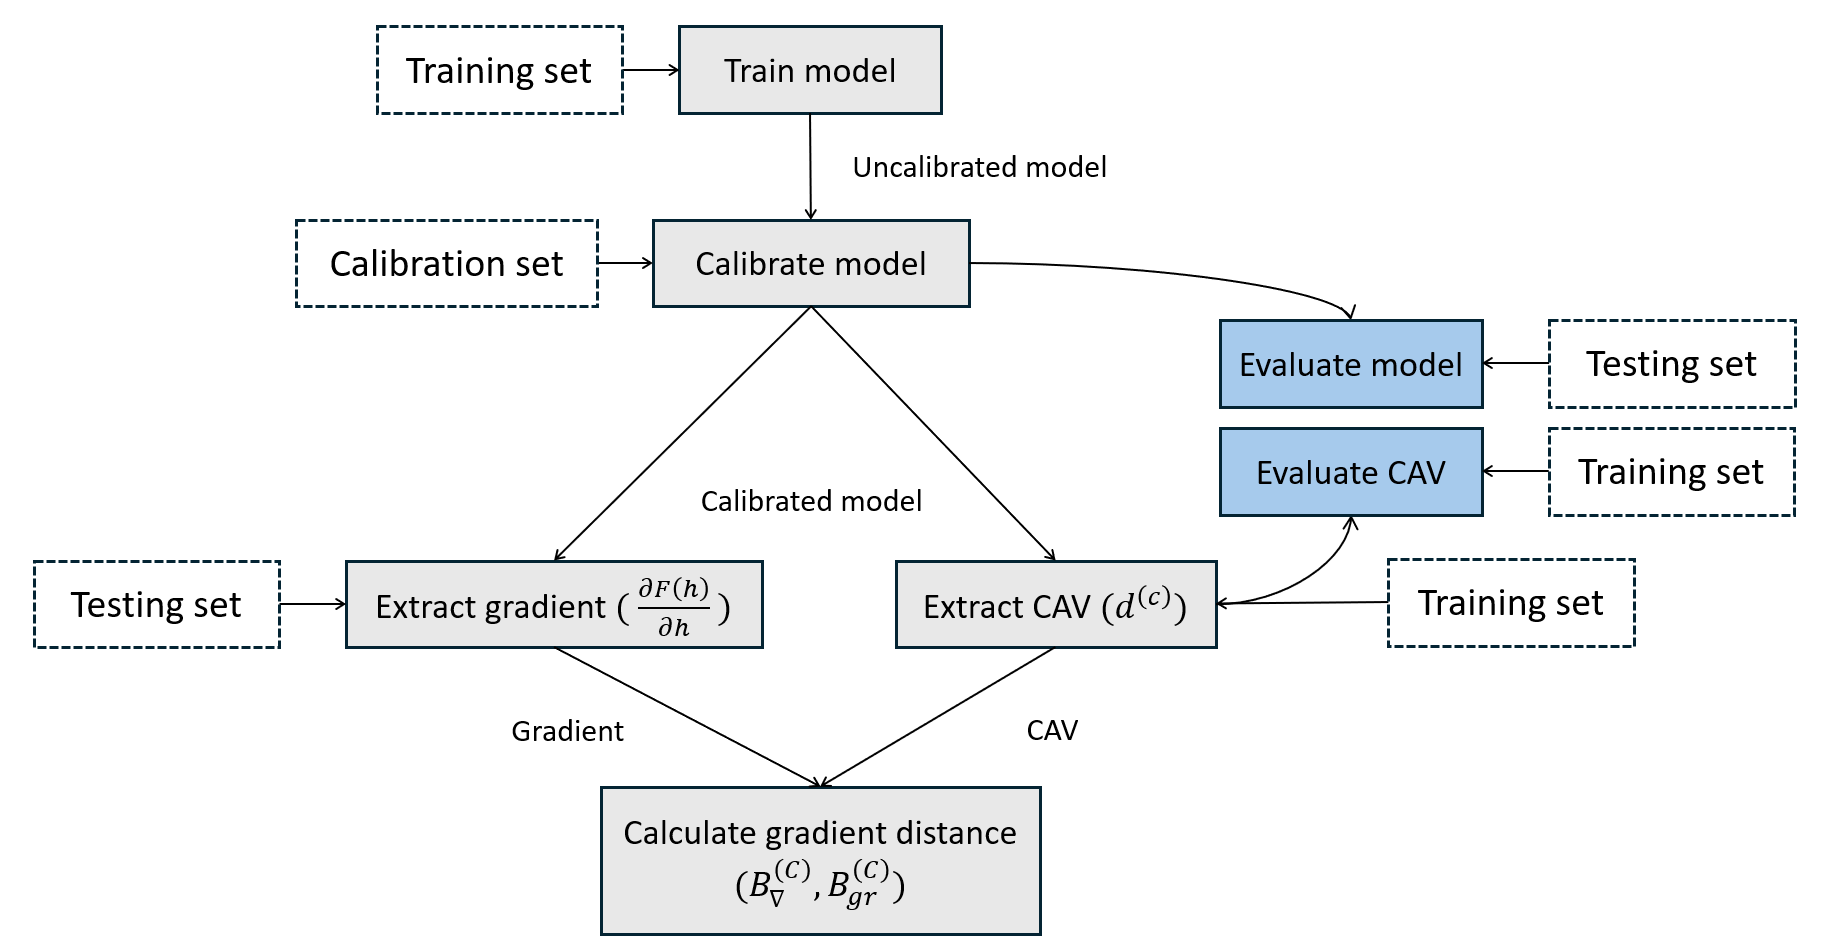
\includegraphics[width=0.95\textwidth]{flow.png}
    \caption{Flow of the process to obtain the bias measurement with gradient distance}
    \label{fig:flow}
\end{figure}

Figure \ref{fig:flow} illustrates the process requires to obtain the bias measurement with gradient distance. The grey boxes represents the main steps of the process. The first step is to train the parameters in the model $\mathcal{F}$, through minimizing the MSE loss function (Equation \ref{eq:mse}) for DNN, and NLL loss function (Equation \ref{eq:nll}) for DDN. Afterwards, the neural network parameters are frozen, and the slope $m$ and intercept $c$ of the subsequent linear regression model (Equation \ref{eq:calibration}) are trained, also through minimizing the MSE loss function. The trained model is then passed with input data, with the gradients $\frac{\partial \mathcal{F}_y}{\partial \boldsymbol{h}}$ and the activation $\boldsymbol{h}$ in the layers tracked for each input. In this experiment, only the gradient and activation from the first layer are investigated. $\boldsymbol{h}$ from all inputs are collected to train a simple linear classifier to differentiate the concept of interest. Through minimizing the hinge-loss function (Equation \ref{eq:hinge-loss}), the CAV $\boldsymbol{d^{(c)}}$ is obtained through the decision boundary. Finally, the gradients $\frac{\partial \mathcal{F}}{\partial \boldsymbol{h}}$ and CAV $\boldsymbol{d^{(c)}}$ are used to calculate the gradient distance $\mathcal{B}^{(c)}_{\nabla}$ (Equation \ref{eq:grad_del}) and $\mathcal{B}^{(c)}_{\nabla}$ (Equation \ref{eq:grad_gr}).

The blue boxes represent the performance evaluation steps that could be done throughout the flow, including the model and the CAV accuracy, using the assessment criteria in section \ref{sec:performance_criteria}.

Finally, the dotted white boxes represent the data used in each step. It refers to where is the source of the intermediate vector $\mathbf{\hat{x}}$ passed into the system $\mathcal{F}$. To highlight, while the testing set is used for model evaluation, the training set is used for CAV evaluation. This choice is made as the CAV evaluation is to measure how accurately the CAV represents the concept during the training process itself.

\section{Hyper-parameters}
\subsection{Model Training}
The model architecture hyper-parameter used for training has been outlined in Chapter \ref{chap:graders}, which includes the layer number, node number, activation function, dropout rate and the model type (DNN vs DDN) hence the minimization function (MSE vs NLL).

All the trainings are done on CUDA with the NVIDIA Tesla V100S-PCIe GPU with 32GB memory, using the PyTorch library. The following explains the training hyper-parameters for each model:

The text-based model is trained for 2 epochs using an Adam optimizer with decoupled weight decay (AdamW) \nomenclature[Z]{AdamW}{Adam Optimizer with Decoupled Weight Decay}. The first and second epochs have a learning rate of $1 \times 10^{-5}$ and $1 \times 10^{-6}$ respectively. The model is trained with a batch size of 8, and the seed number is set to 5. Each seed's training process takes approximately 2 hours.

The feature-based model is trained for 200 epochs using an Adam optimizer with a learning rate of $1 \times 10^{-5}$. The model is trained with a batch size of 20, and the seed number is also set to 5. Each seed's training process also takes approximately 2 hours.

The audio-based model is trained for 4 epochs using an AdamW optimizer, which has a learning rate of $1 \times 10^{-6}$. The model is trained with a batch size of 32, and the seed number is set to 2, less than that of text and feature-based model. It is because the training process for each seed takes approximately 36 hours, hence it is computationally more feasible to compare with less seeds.


Table \ref{tab:training_hyper_param} summarizes the training hyper-parameters for each model.

\begin{table}[H]
    \centering
    \begin{tabular}{|l|c|c|c|}
        \hline
                                  & \textbf{Text-Based}                             & \textbf{Feature-Based} & \textbf{Audio-Based} \\
        \hline
        \textbf{Optimizer}        & AdamW                                           & Adam                   & AdamW                \\ \hline
        \textbf{Learning Rate}    & $1 \times 10^{-5} \rightarrow 1 \times 10^{-6}$ & $1 \times 10^{-5}$     & $1 \times 10^{-6}$   \\ \hline
        \textbf{Epochs}           & 2                                               & 200                    & 4                    \\ \hline
        \textbf{Batch Size}       & 8                                               & 20                     & 32                   \\ \hline
        \textbf{Seed number}      & 5                                               & 5                      & 2                    \\ \hline
        \textbf{Duration (hours)} & 2                                               & 2                      & 36                   \\ \hline
    \end{tabular}
    \caption{Training hyper-parameters for different model types}
    \label{tab:training_hyper_param}
\end{table}

\subsection{CAV Linear Classifier Training}
The CAV linear classifier follows the one implemented in \cite{feature_bias}. The regularization parameter $\alpha$ in equation \ref{eq:hinge-loss}, which controls the strength of L2-norm penalty, used a value of 0.001. Stochastic Gradient Descent is used as the optimizer, with the learning rate scheduled optimally using implementation from \verb|Scikit-learn| \cite{scikit-learn}. The training step is limited with 2000 iterations, and it steps when the MSE change is within $1 \times 10^{-4}$. Polyak–Ruppert averaging is used, which means the last 16 sets of CAV weights and bias are averaged as the output. The CAV is extractable within minutes.

\section{Model Biasing}
To understand how effective the bias measurement with CAV is, a biased model is trained through feeding in training data deliberately biased towards a specific concept. The biased model would also follow the same flow as the original model to calculate the gradient distance $\mathcal{B}^{(c)}_{\nabla}$ and $\mathcal{B}^{(c)}_{gr}$. The results are used to compare with the original model. If the original model is unbiased, and $\mathcal{B}^{(c)}_{\nabla}$ and $\mathcal{B}^{(c)}_{gr}$ could reflect the bias, it is expected that $\mathcal{B}^{(c)}_{\nabla}$ and $\mathcal{B}^{(c)}_{gr}$ of the concept being biased would still be close to 1 for the original model, but deviate from 1 for the biased one.

To bias the training data, all positive targets of the concept under consideration have their predicted score increased by 1. A maximum cap of 6 is applied for the increment, such that the scores would not exceed the maximum score of the exam.

\section{Factor Isolation}
Plotting the results of the bias measurement with individual candidates' gradient distance $\mathcal{B}^{(ci)}_{gr}$ against their predicted score, it is observed that feature-based models are more sensitive to bias measurement. To understand what factors are affecting $\mathcal{B}^{(ci)}_{gr}$'s pattern, particularly its sensitivity to bias measurement, the models are trained with different hyper-parameters, and their bias measurements are compared with the original models to isolate the factors. Text and feature-based models are chosen for comparison, as both text and audio-based models are based on the attention mechanism, while feature-based model is not. Between text and audio model, text-based model takes less time to train and evaluate, hence it is chosen for comparison.

The first factor considered is the network architecture. It is hypothesized that the layer number and node number would affect the pattern of $\mathcal{B}^{(ci)}_{gr}$. Hence, a new feature-based model is trained in Figure \ref{fig:bert_like}, but with the layer number, node number and dropout rate same as that of the text-based mode. The unchanged and changed components are in blue and red respectively. The input remains 356-dimensional for the feature vector, and the output remains 2-dimensional for the Gaussian mean $\mu$ and standard deviation $\sigma$ prediction. The activation function is also kept as LReLU.

\begin{figure}[H]
    \centering
    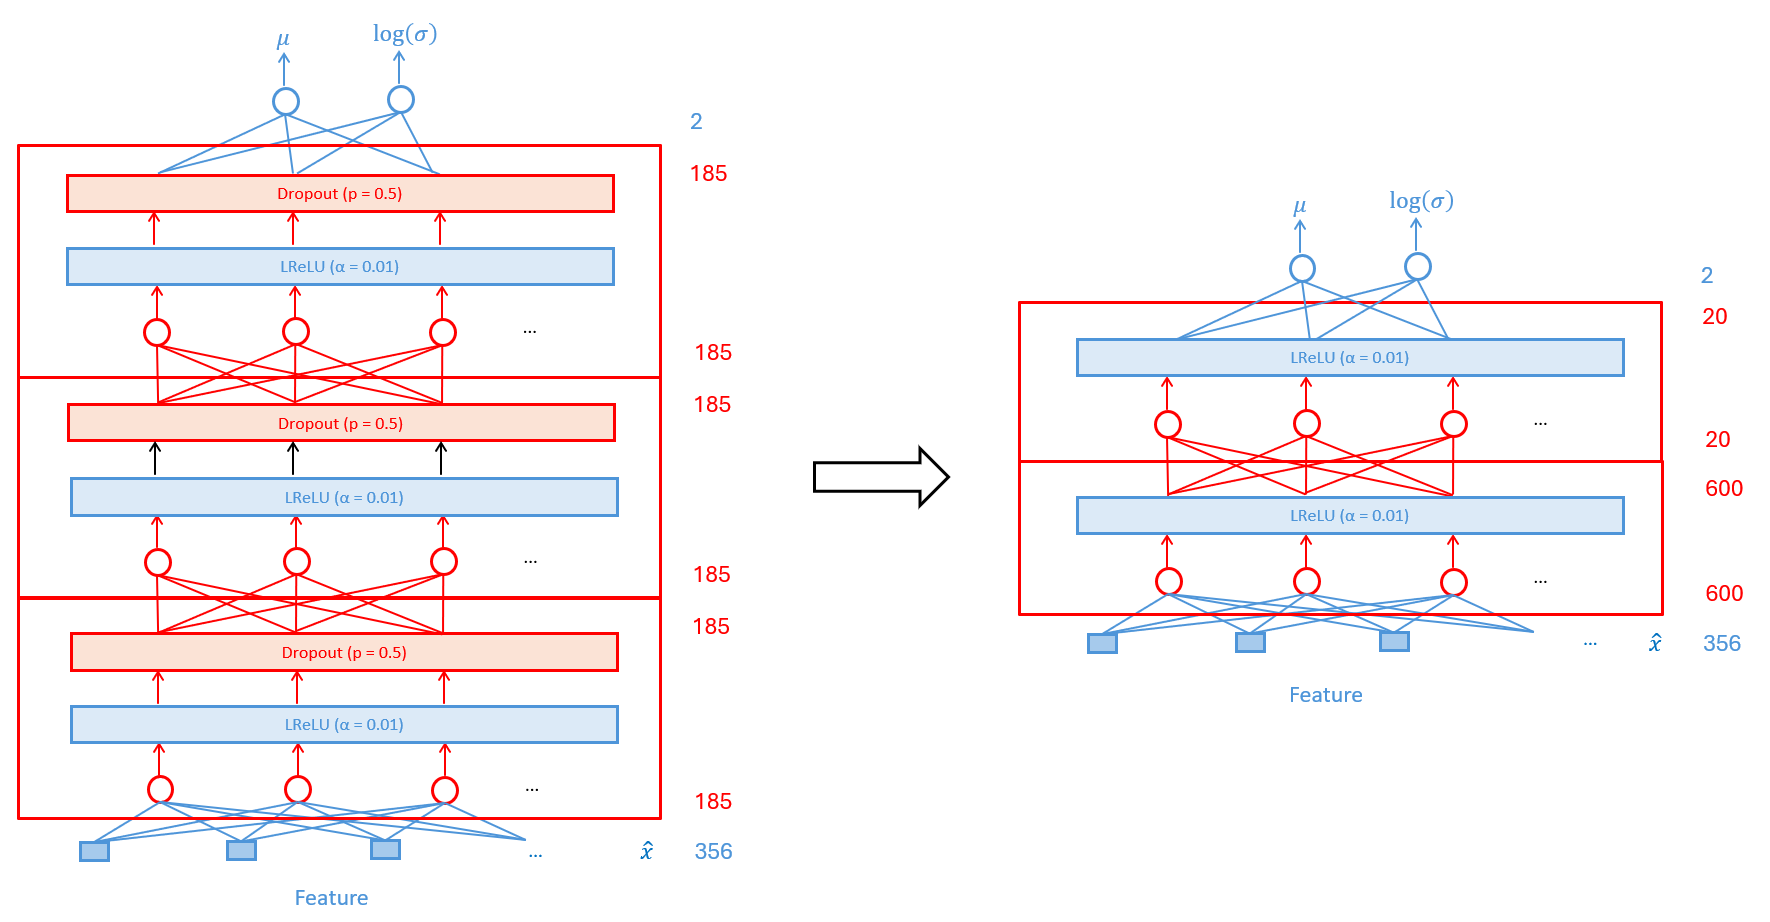
\includegraphics[width=0.85\textwidth]{bert_like.png}
    \caption{Change of feature-based model architecture similar to text-based model, with original (left) and new (right) architecture}
    \label{fig:bert_like}
\end{figure}

The second factor considered is the model type. It is hypothesized that the use of DNN would affect the pattern of $\mathcal{B}^{(ci)}_{gr}$. Hence, a new feature-based model is trained in figure \ref{fig:dnn_like}, but with the model type changed from DDN to DNN, while keeping the model architecture same as that of the original feature-based model. The loss function is subsequently also changed from MSE to NLL.

\begin{figure}[H]
    \centering
    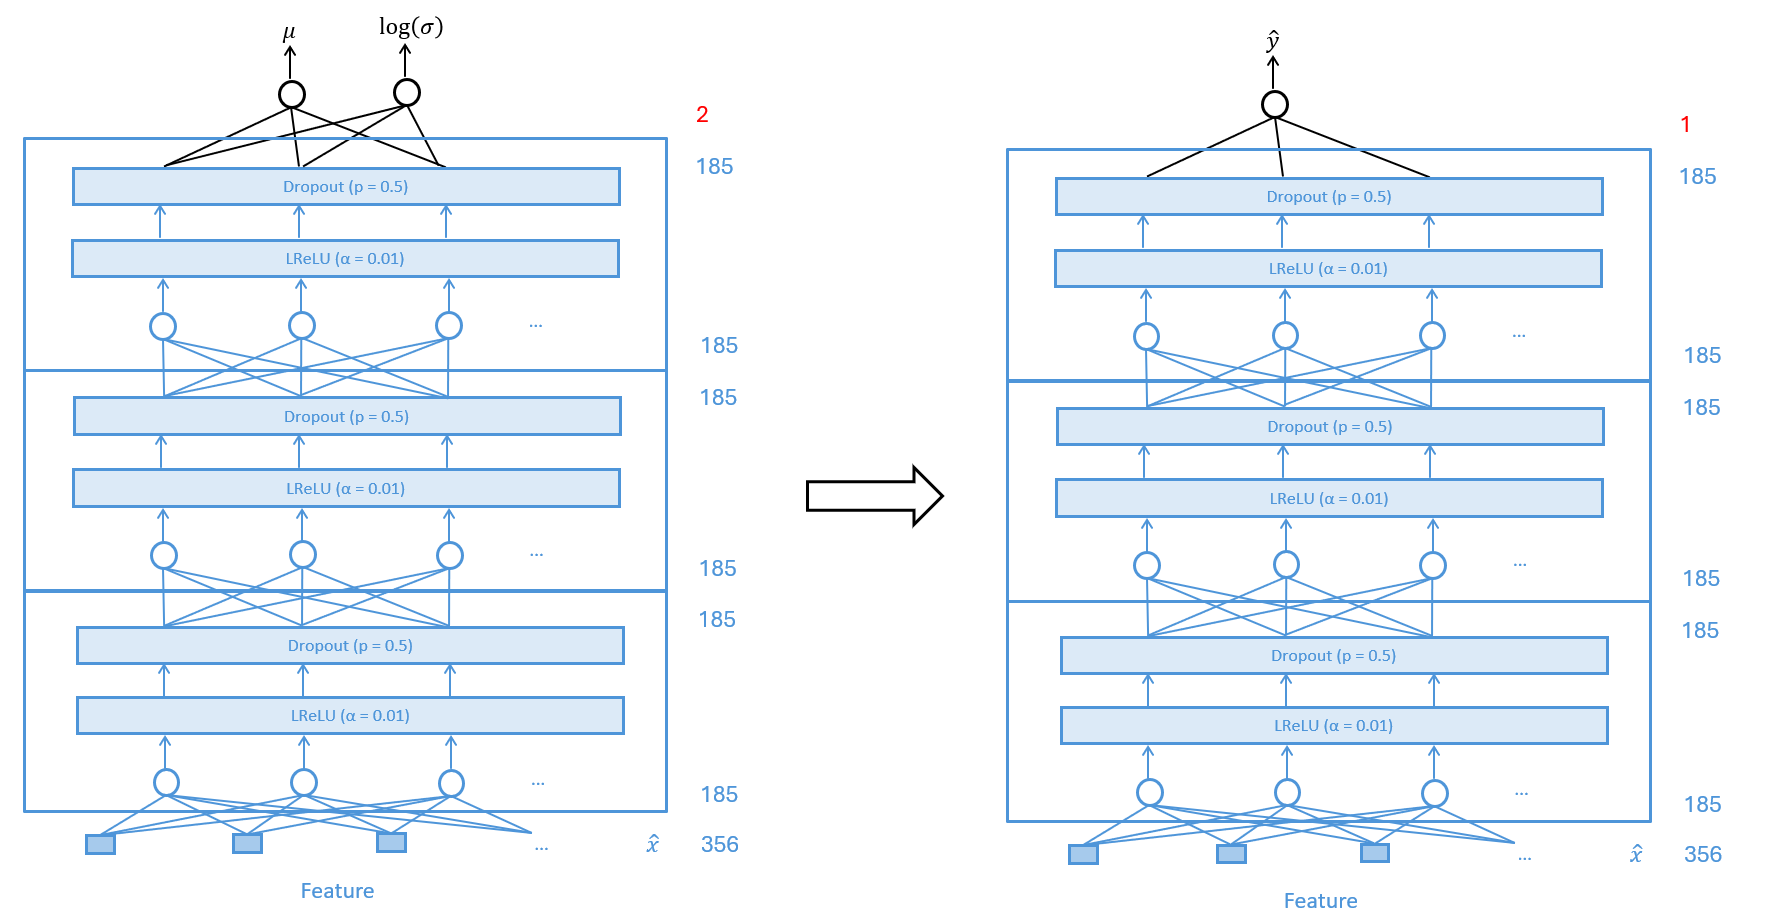
\includegraphics[width=0.85\textwidth]{dnn_like.png}
    \caption{Change of feature-based model from DDN (left) to DNN (right)}
    \label{fig:dnn_like}
\end{figure}

The third factor is the activation function. It is hypothesized that the use of LReLU would affect the pattern of $\mathcal{B}^{(ci)}_{gr}$. Hence, a new feature-based model is trained in figure \ref{fig:relu}. The activation function changed from LReLU to ReLU, which is the activation function used in the text and audio-based model. The model architecture is kept the same as that of the original feature-based model, and the loss function is kept as NLL.

\begin{figure}[H]
    \centering
    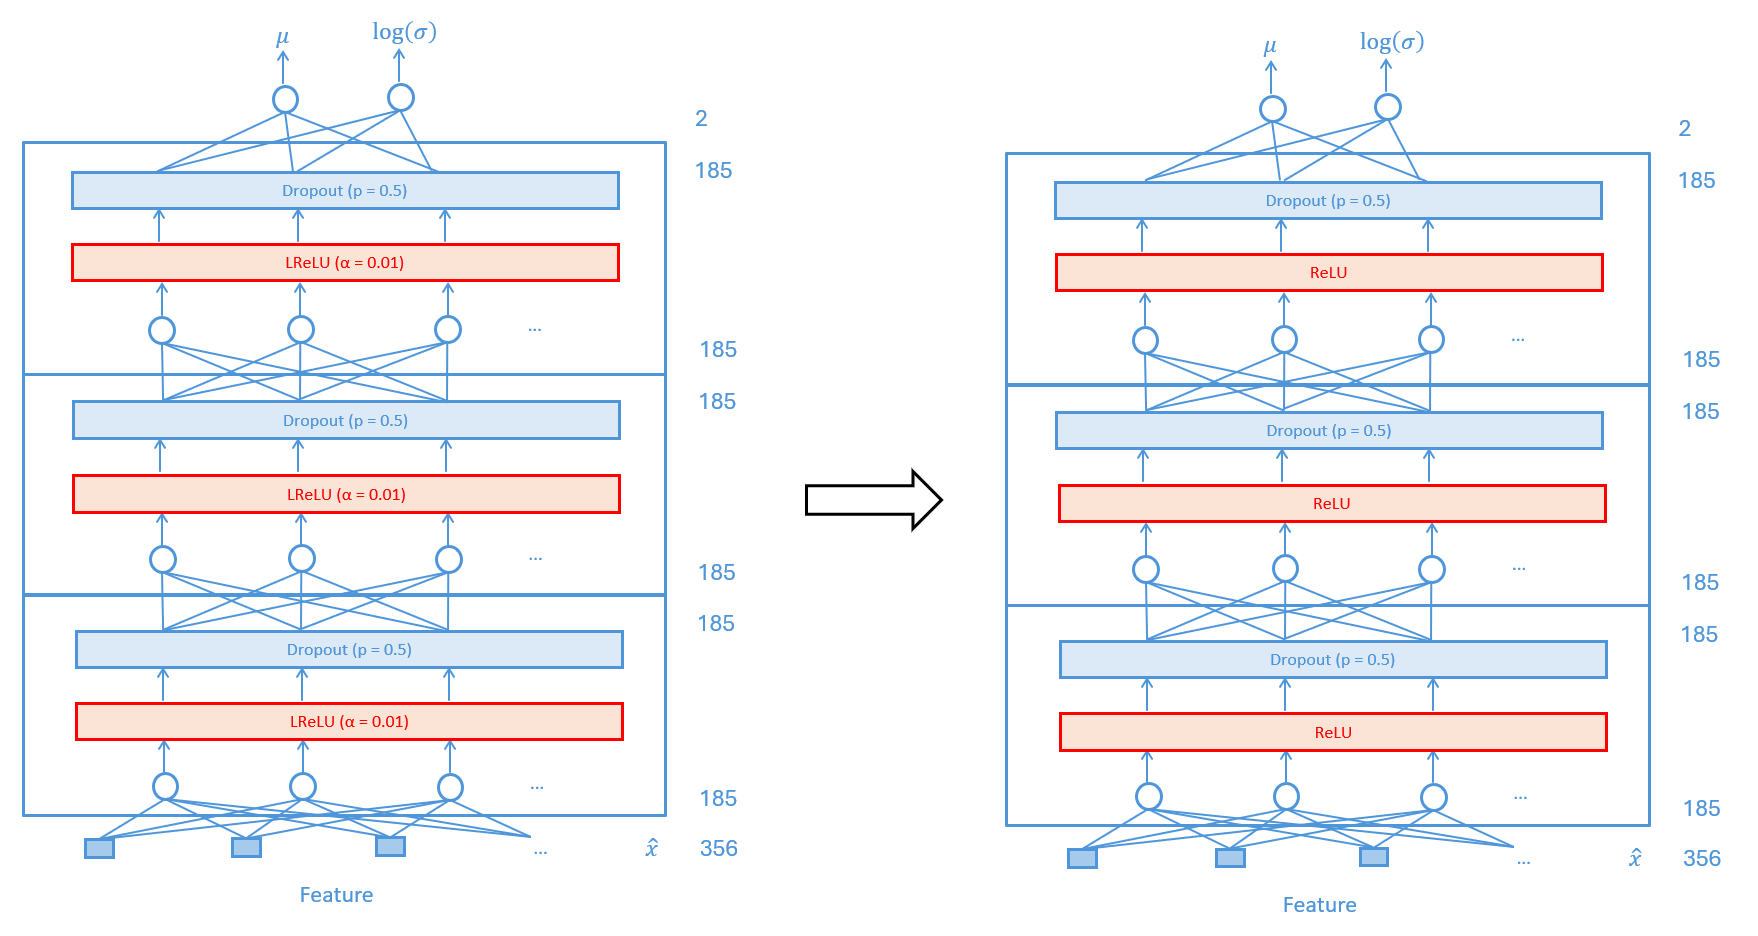
\includegraphics[width=0.85\textwidth]{relu.png}
    \caption{Change of feature-based model activation function from LReLU (left) to ReLU (right)}
    \label{fig:relu}
\end{figure}

In addition, a new text-based model is trained in figure \ref{fig:lrelu}, with the activation function changed from ReLU to LReLU, which is the activation function used in the feature-based model. The model architecture is kept the same as that of the original text-based model, and the loss function is kept as MSE.

\begin{figure}[H]
    \centering
    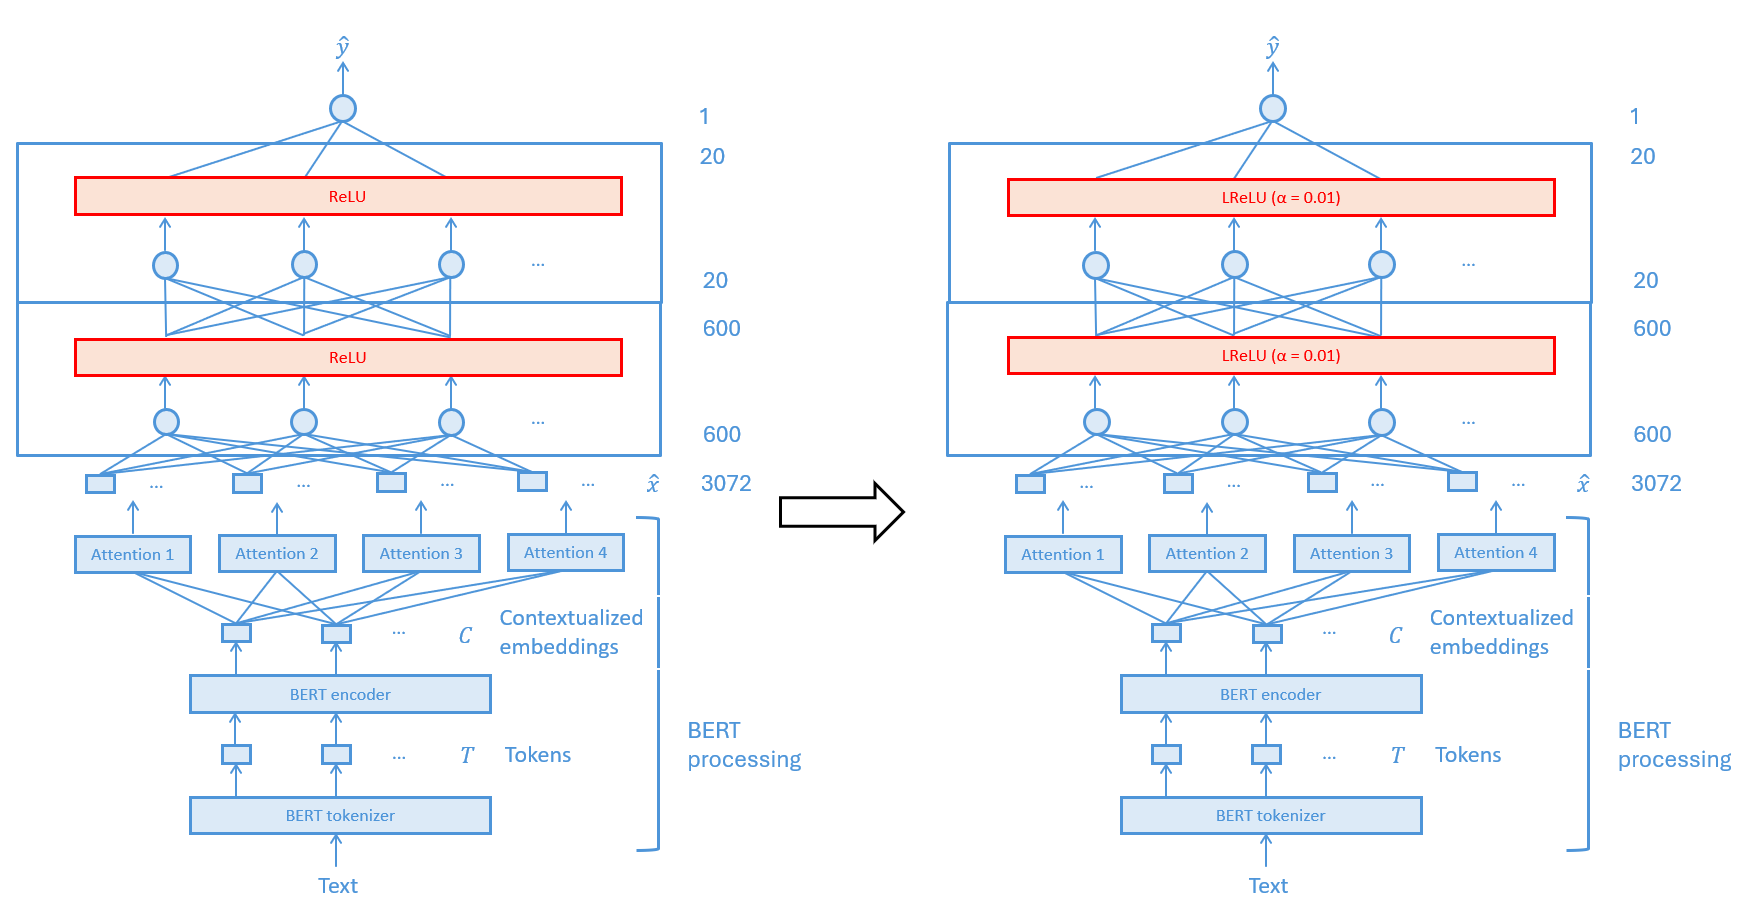
\includegraphics[width=0.85\textwidth]{lrelu.png}
    \caption{Change of text-based model activation function from ReLU (left) to LReLU (right)}
    \label{fig:lrelu}
\end{figure}

The fourth factor is the input. It is hypothesized that the nature of the input, whether it is vectors generated from attention mechanism, or feature vectors, would affect pattern of $\mathcal{B}^{(ci)}_{gr}$. Hence, the text-based model is modified to concatenate the attention embeddings $\mathbf{\hat{x}}$ with the feature vector, before passing it into the neural network. The network architecture remains the same as the text-based model, except the input dimension is now $3072 + 356 = 3428$-dimensional. The feature vector would only contribute to $10.4\%$ of the concatenated input vector, which is a rather small proportion only. The modification is shown in figure \ref{fig:deep_fusion}.

\begin{figure}[H]
    \centering
    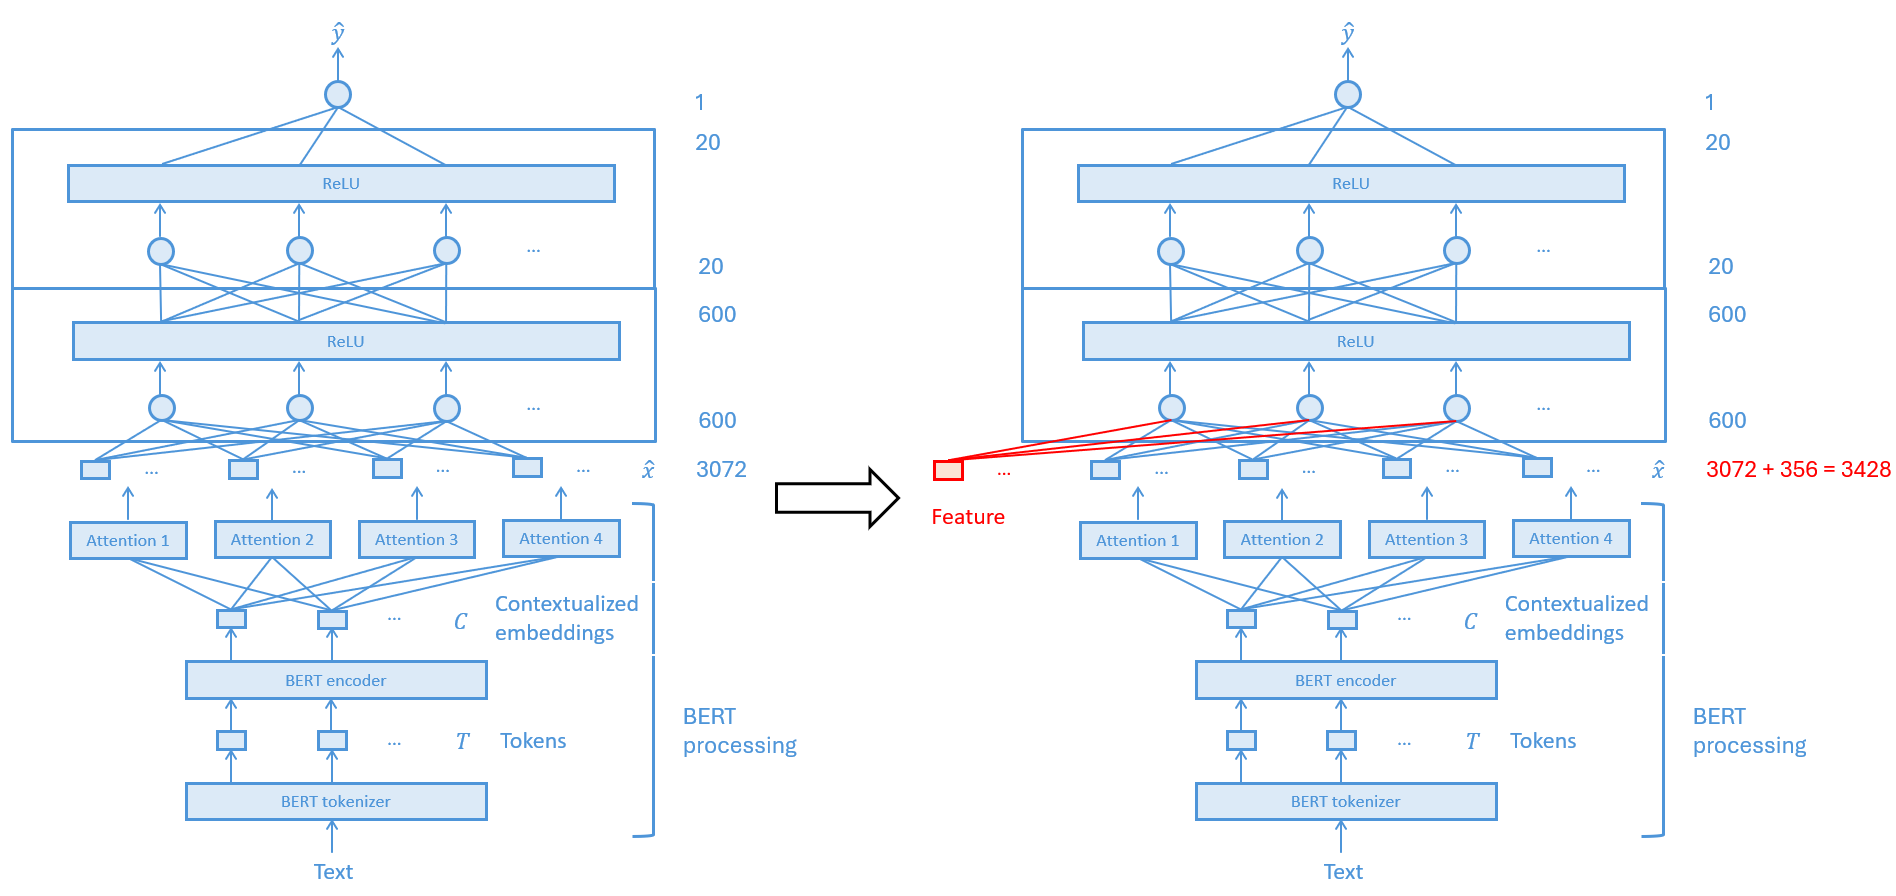
\includegraphics[width=0.85\textwidth]{deep_fusion.png}
    \caption{Deep fusion of feature vector and BERT attention embeddings, with original (left) and new (right) input method}
    \label{fig:deep_fusion}
\end{figure}

\section{Performance Criteria} \label{sec:performance_criteria}
\subsection{Model Performance}
The model's performance is evaluated with four criteria: the root mean square error (RMSE) and the Pearson correlation coefficient (PCC) \nomenclature[Z]{PCC}{Pearson Correlation Coefficient} between the predicted scores and the human graders' scores, the percentage of scores within 0.5 of the human graders' scores ($< 0.5$),  \nomenclature[Z]{$< 0.5$}{Percentage of Scores Within 0.5 of Human Graders'} and the percentage of scores within 1 of the human graders' scores ($< 1$) \nomenclature[Z]{$< 1$}{Percentage of Scores Within 1 of Human Graders'}.

The RMSE is calculated using Equation \ref{eq:rmse}, which is used to measure the accuracy of the model's predictions. A lower RMSE is desired as it indicates the model's prediction is closer to the actual scores given by the human graders.

\begin{equation} \label{eq:rmse}
    \text{RMSE} = \sqrt{\frac{1}{n} \sum_{i=1}^{n} (y_i - \hat{y}_i)^2}
\end{equation}

The PCC is calculated using Equation \ref{eq:pcc}, which measures the linear correlation between the predicted scores and the actual scores. A PCC value close to 1 indicates a strong positive correlation, a value close to -1 indicates a strong negative correlation, and a value close to 0 indicates no correlation. A PCC value closer to 1 is preferred, as it indicates that the model's predictions are closely aligned with the human graders' scores.

\begin{equation} \label{eq:pcc}
    \text{PCC} = \frac{\sum_{i=1}^{n} (y_i - \bar{y})(\hat{y}_i - \bar{\hat{y}})}{\sqrt{\sum_{i=1}^{n} (y_i - \bar{y})^2} \sqrt{\sum_{i=1}^{n} (\hat{y}_i - \bar{\hat{y}})^2}}
\end{equation}

where $y_i$ is the actual score given by the human graders, $\hat{y}_i$ is the predicted score by the model, $\bar{y}$ is the mean of the actual scores, and $\bar{\hat{y}}$ is the mean of the predicted scores.

For the percentage of scores within 0.5 and 1 of the human graders' scores, the percentage is calculated using Equation \ref{eq:within_05} and \ref{eq:within_1} respectively, where $n$ is the total number of candidates, and $y_i$ is the actual score given by the human graders, while $\hat{y}_i$ is the predicted score by the model. A higher percentage indicates that the model's predictions are closer to the human graders' scores, which is desired.

\begin{equation} \label{eq:within_05}
    \text{Percentage of Scores Within 0.5} = \frac{1}{n} \sum_{i=1}^{n} \mathbb{I}(|y_i - \hat{y}_i| < 0.5)
\end{equation}

\begin{equation} \label{eq:within_1}
    \text{Percentage of Scores Within 1} = \frac{1}{n} \sum_{i=1}^{n} \mathbb{I}(|y_i - \hat{y}_i| < 1)
\end{equation}
where $\mathbb{I}$ is the indicator function, which returns 1 if the condition is true, and 0 otherwise.

\subsection{CAV Performance}
The performance of CAV is evaluated with the accuracy of the linear classifier, which is trained to differentiate the concept of interest. The positive and negative target accuracy is calculated using Equation \ref{eq:pos_accuracy} and \ref{eq:neg_accuracy} respectively, where $TP$ is the number of true positives, $TN$ is the number of true negatives, $FP$ is the number of false positives, and $FN$ is the number of false negatives.

\begin{equation} \label{eq:pos_accuracy}
    \text{Positive Target Accuracy} = \frac{TP}{TP + FP}
\end{equation}

\begin{equation} \label{eq:neg_accuracy}
    \text{Negative Target Accuracy} = \frac{TN}{TN + FN}
\end{equation}

\subsection{Bias Measurement}
As mentioned in Section \ref{sec:gradient}, the bias measurement is calculated using the gradient distance $\mathcal{B}^{(c)}_{\nabla}$ and $\mathcal{B}^{(c)}_{gr}$. A plot of $\mathcal{B}^{(ci)}_{gr}$ against individual candidates' score could also be plotted. The bias measurement is expected to be close to 1 for an unbiased model, and deviate from 1 for a biased model. Hence, if the gap between the gradient distance between the biased and unbiased model is significant, it indicates that the bias measurement is effective in measuring the bias in the model.

\section{Summary}
This chapter outlines the data and experimental setup used in this study. The dataset is constructed from responses of candidates taking the Linguaskill exams, divided into training, calibration, and testing sets. The process of training, calibration, and testing is described, along with the hyper-parameters used for model training and CAV extraction. The chapter also discusses the model biasing process and factor isolation to understand the impact of different components on the bias measurement. Finally, the performance criteria for evaluating the model and CAV are defined.